\documentclass[pdftex,12pt,a4paper]{article}

\usepackage{graphicx}  
\usepackage[margin=2.5cm]{geometry}
\usepackage{breakcites}
\usepackage{indentfirst}
\usepackage{pgfgantt}
\usepackage{pdflscape}
\usepackage{float}
\usepackage{epsfig}
\usepackage{epstopdf}
\usepackage[cmex10]{amsmath}
\usepackage{stfloats}
\usepackage{multirow}

\renewcommand{\refname}{REFERENCES}
\linespread{1.3}

\usepackage{mathtools}
%\newcommand{\HRule}{\rule{\linewidth}{0.5mm}}
\thispagestyle{empty}
\begin{document}
\begin{titlepage}
\begin{center}
\textbf{}\\
\textbf{\Large{ISTANBUL TECHNICAL UNIVERSITY}}\\
\vspace{0.5cm}
\textbf{\Large{COMPUTER ENGINEERING DEPARTMENT}}\\
\vspace{2cm}
\textbf{\Large{BLG 222E\\ Computer Organization \\ Project 1}}\\
\vspace{2.8cm}
\begin{table}[ht]
\centering
\Large{
\begin{tabular}{lcl}
\textbf{PROJECT DATE}  & : & 24.05.2023\\
\end{tabular}}
\end{table}
\vspace{1cm}
\textbf{\Large{GROUP MEMBERS:}}\\
\begin{table}[ht]
\centering
\Large{
\begin{tabular}{rcl}
150220762  & : & Muhammed Yusuf Mermer (Group Representative)  \\
150210071  & : & Emre Çamlıca \\
150200091  & : & Hakan Duran \\
\end{tabular}}
\end{table}
\vspace{2.8cm}
\textbf{\Large{SPRING 2023}}

\end{center}

\end{titlepage}

\thispagestyle{empty}
\addtocontents{toc}{\contentsline {section}{\numberline {}FRONT COVER}{}}
\addtocontents{toc}{\contentsline {section}{\numberline {}CONTENTS}{}}
\setcounter{tocdepth}{4}
\tableofcontents
\clearpage

\setcounter{page}{1}
\section{INTRODUCTION}
In this project our purpose was to design a hardwired control unit. To achive 
this we firstly implemented small components of this system. Yusuf did the fetch and decode parts, Hakan did the instructions without memory reference and Emre did the instructions with memory reference. Yusuf also wrote the test bench and tested the system with Hakan.

At first, Yusuf has designed the fetch cycle. Then Hakan and Emre designed the execute part. Hakan and Yusuf then tested the project and corrected the errors.


\section{IMPLEMENTATIONS AND EXPLANATIONS }
\subsection{Fetch Cycle, Counter and Decoding}
In our implementations, we made only counter module seperated from the 
combined system. It could have also been designed inside of overall 
combined system as a register, but this was our design choice. It takes 
clock as input, because at every positive edge we increase our timing signal
by 1. However, to prevent unexpected result in the current postive edge we wait for
0.25 ns in our implementation.

Not only clock, but also reset signal taken as input for this module
to return inital value for the timing signal. When it reset, it returns value 4 bit
binary 1111 which is equal to -0001, this is been made because reset signal 
does not depend on clock; therofore, after the reset we wait for new clock signal 
to start new operations. New operations will be started with timing signal 0.

Inside of inital block, we make all register values 0 for use in the operations.
Then to prevent further changes we closed rsel and tsel values.

We have 3 always block inside of our implementations. Our very first always
 block works at every new instruction. It closes all rsels and tsels and also
 closes IR enable. Also after reseting signal, we need to make reset command
 0 to prevent always 0 problem of counter.

2nd always block, works similar to 1st one but it doesn't reset at every time,
because this operation doesn't needed. In here our purpose is to close all
registers from changing their values with the incoming new timing signal.


After making all necesessary connections, in 3rd always block, when timing signal 0 
arrives to our combined system, it starts to fetch cycle. Our 
fetch cycle is totally takes 3 cycles. It has been made 3 cycles to prvent 
changes unintended changes on the PC and IR.



At first (0th) cycle of the fetch, we just pushed values of M[PC] to the IR's LS 8 bits.
This because memory can only give 8 bit output at once. To do this operation, we give PC
as adress to memory.

At second (1st) cycle, we only increased PC value by one. To do this, we just opened PC's
register for input changes and send increment by one signal to funsel of arf.

At last (2nd) cycle, we do combined operations of 0th and 1st cyles, but different than 0th,
this time high bits of IR will be changed.



For decoding part (3th cycle), for the opcodes that addresing mode doesn't requried, we made a simple output opener.
In other words, our module looks at here to decide where to take sreg's. It depends on the where register resits. If [2] bit
is 0 it means that it will be RF, if 1 it will be ARF. The pattern of RF same for [1:0], so we did not
make a change end send them directly. However for ARF, we used switch case for manipulation.


At the end of every insturction, we need to send a reset signal, so depending 
on the opcode type, we will send request for reset. When all operations are finished 
for a instuction, this operations occurs in the next clock cycle.






\subsection{Instructions With Address Reference}

\subsection{Instructions Without Address Reference}






\section{OVERALL DESIGN PHOTO}


\begin{figure}[H]
    \centering
    \includegraphics[width=1\textwidth]{photos/design.png}	
    \caption{overall design photo}
    \label{implementation}
\end{figure}








\section{SIMULATION RESULTS}


\begin{figure}[H]
    \centering
    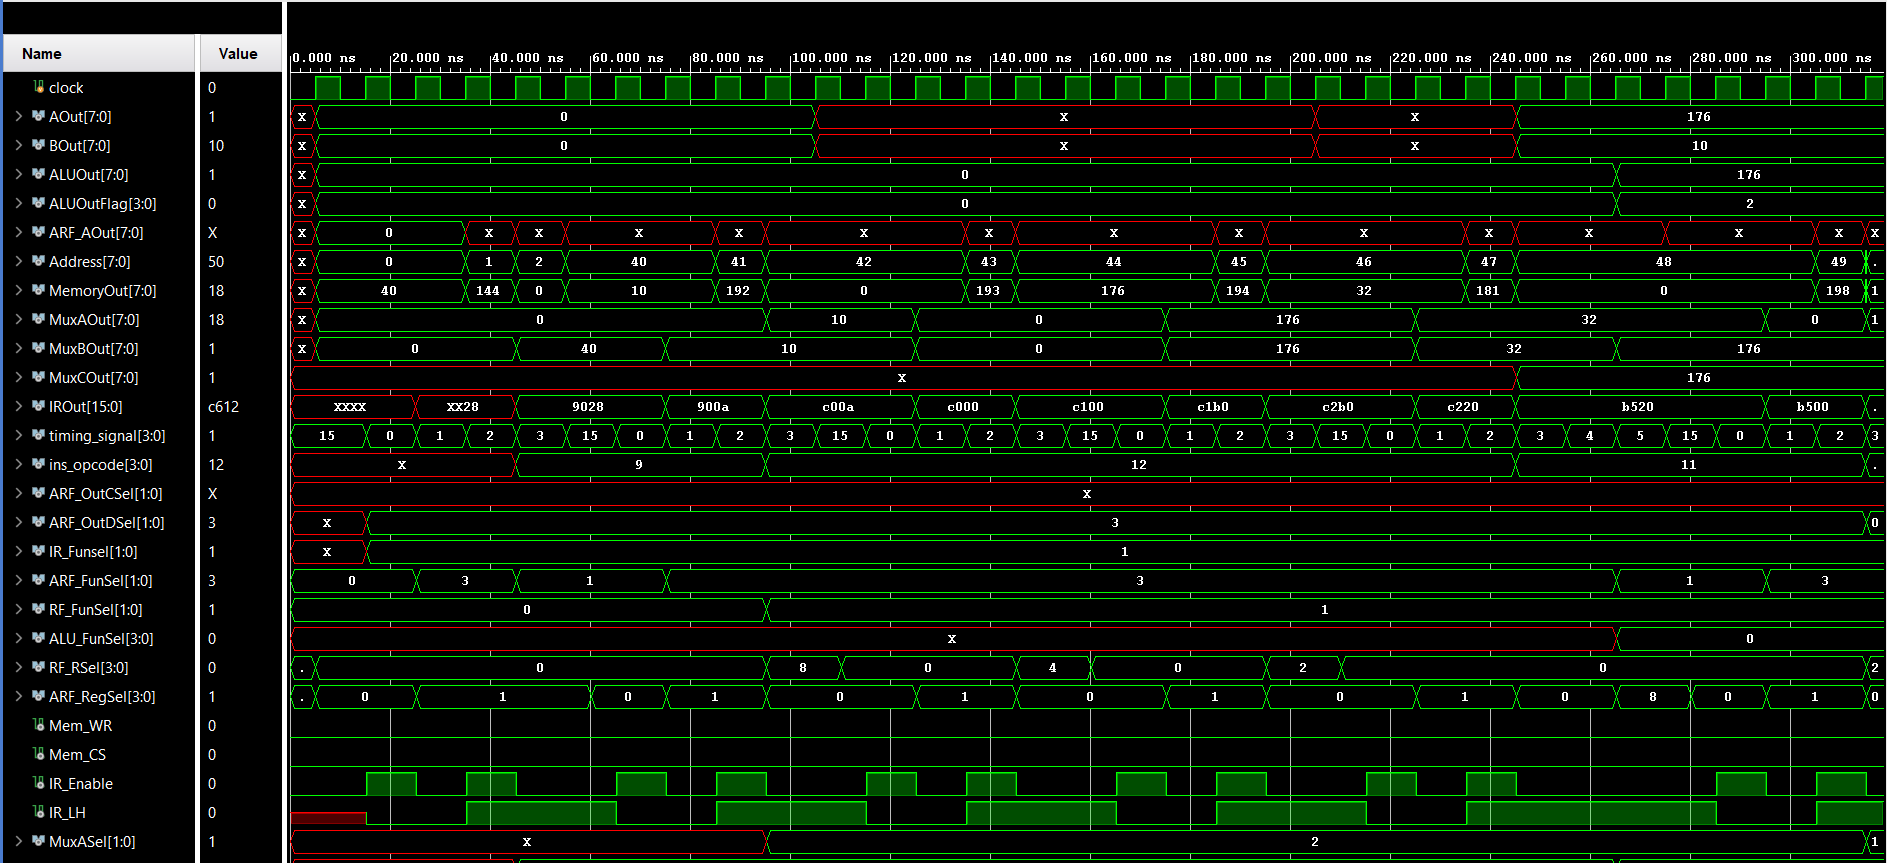
\includegraphics[width=1\textwidth]{photos/system_result_1.png}	
    \caption{simulation of system}
    \label{implementation}
\end{figure}


\begin{figure}[H]
    \centering
    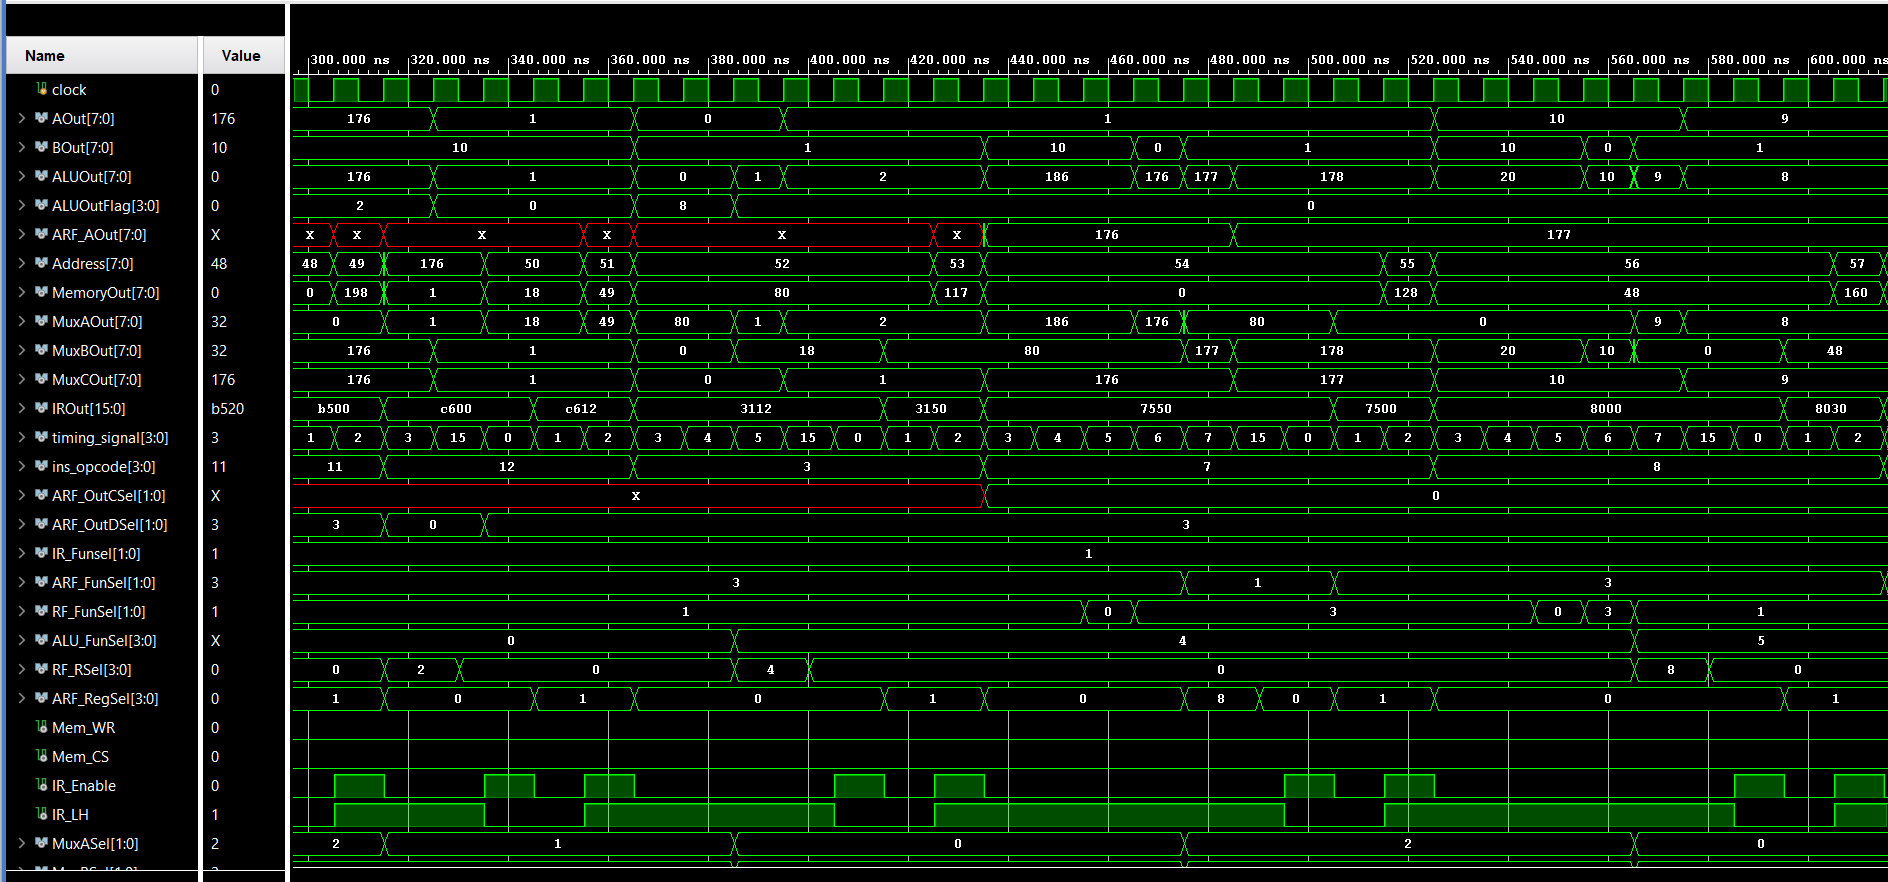
\includegraphics[width=1\textwidth]{photos/system_result_2.png}	
    \caption{simulation of system}
    \label{implementation}
\end{figure}


\begin{figure}[H]
    \centering
    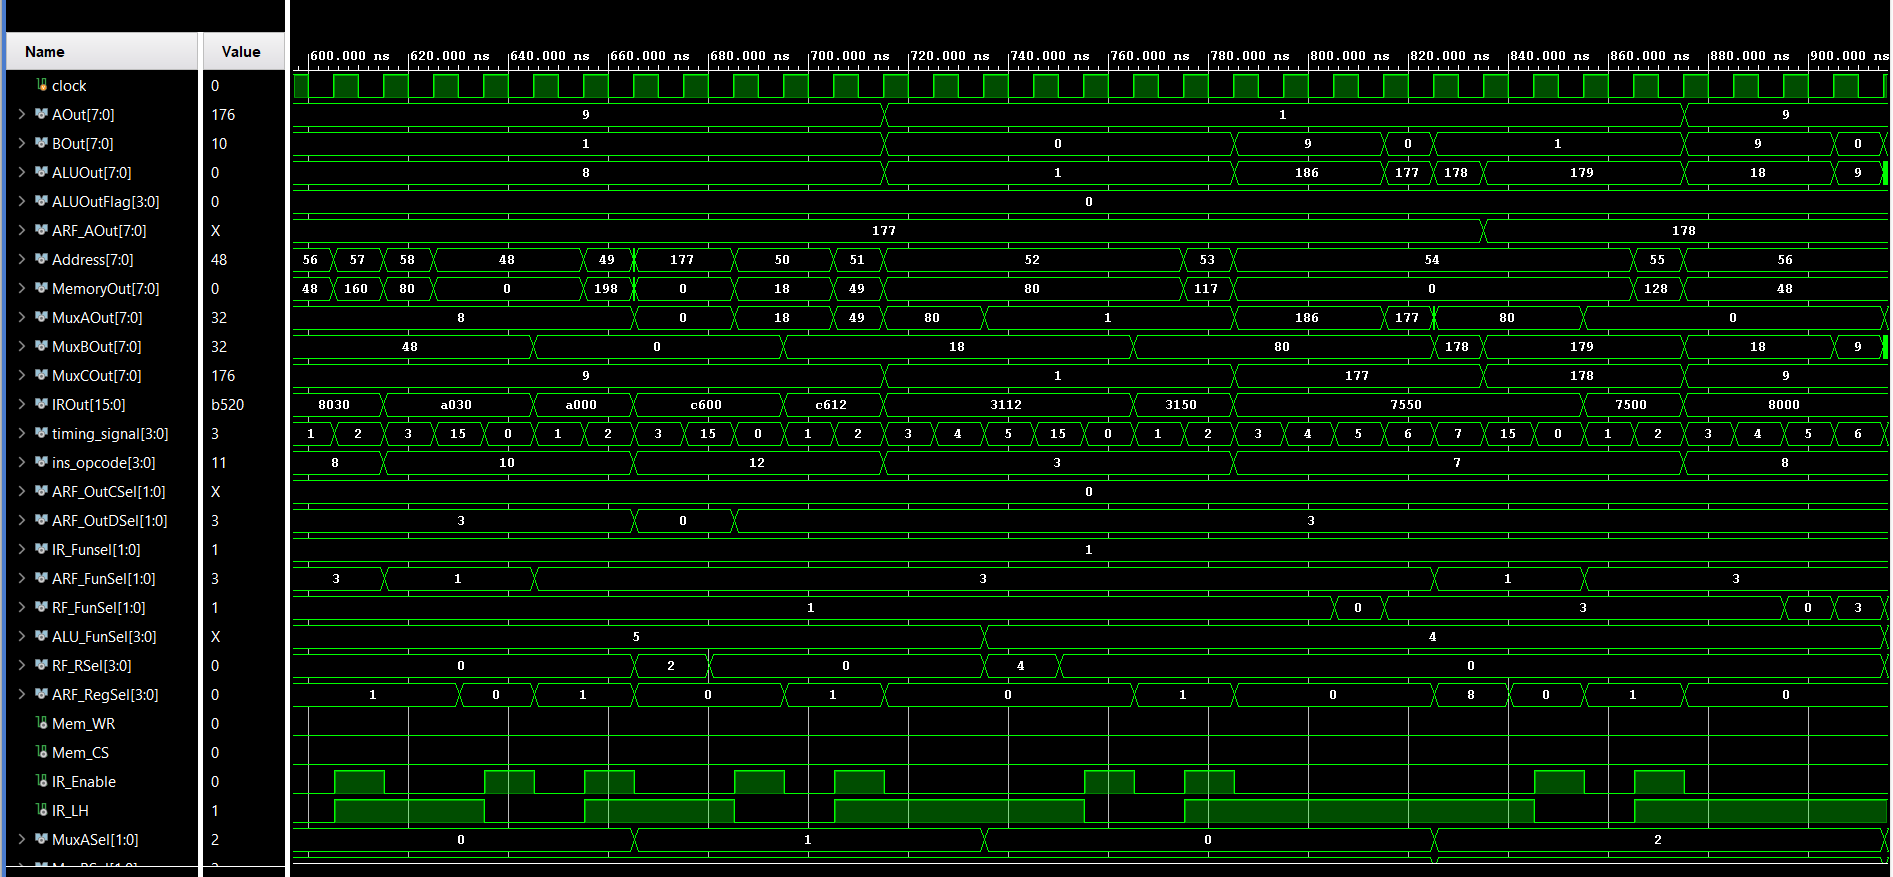
\includegraphics[width=1\textwidth]{photos/system_result_3.png}	
    \caption{simulation of system}
    \label{implementation}
\end{figure}



\begin{figure}[H]
    \centering
    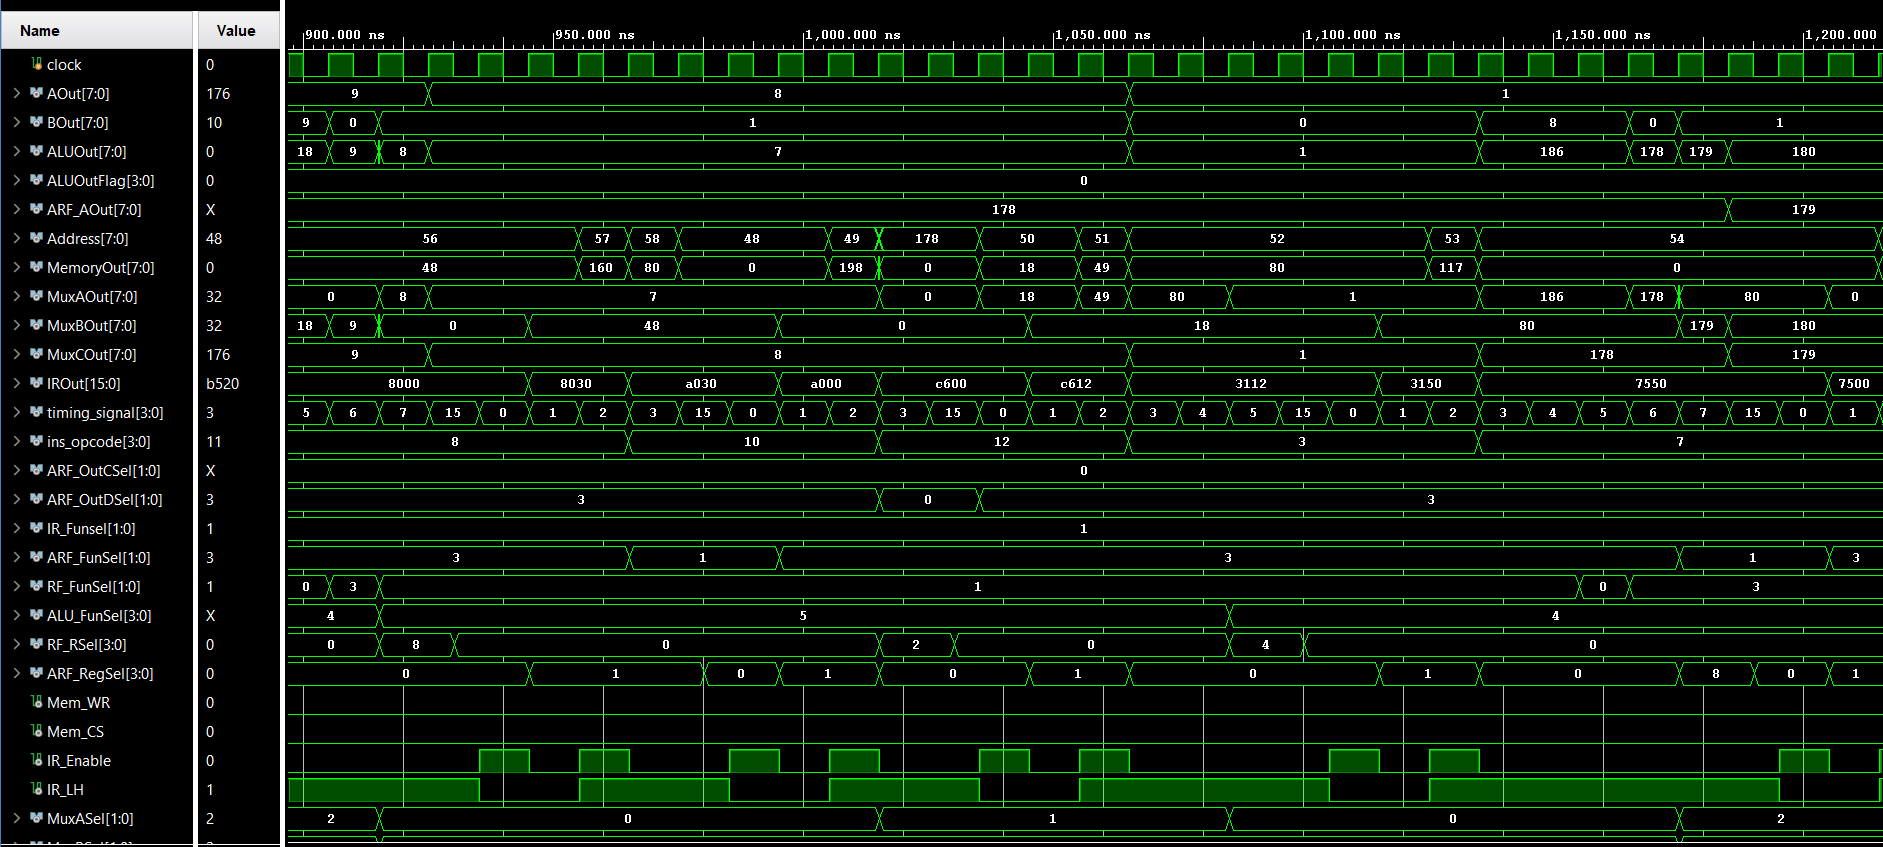
\includegraphics[width=1\textwidth]{photos/system_result_4.png}	
    \caption{simulation of system}
    \label{implementation}
\end{figure}

\begin{figure}[H]
    \centering
    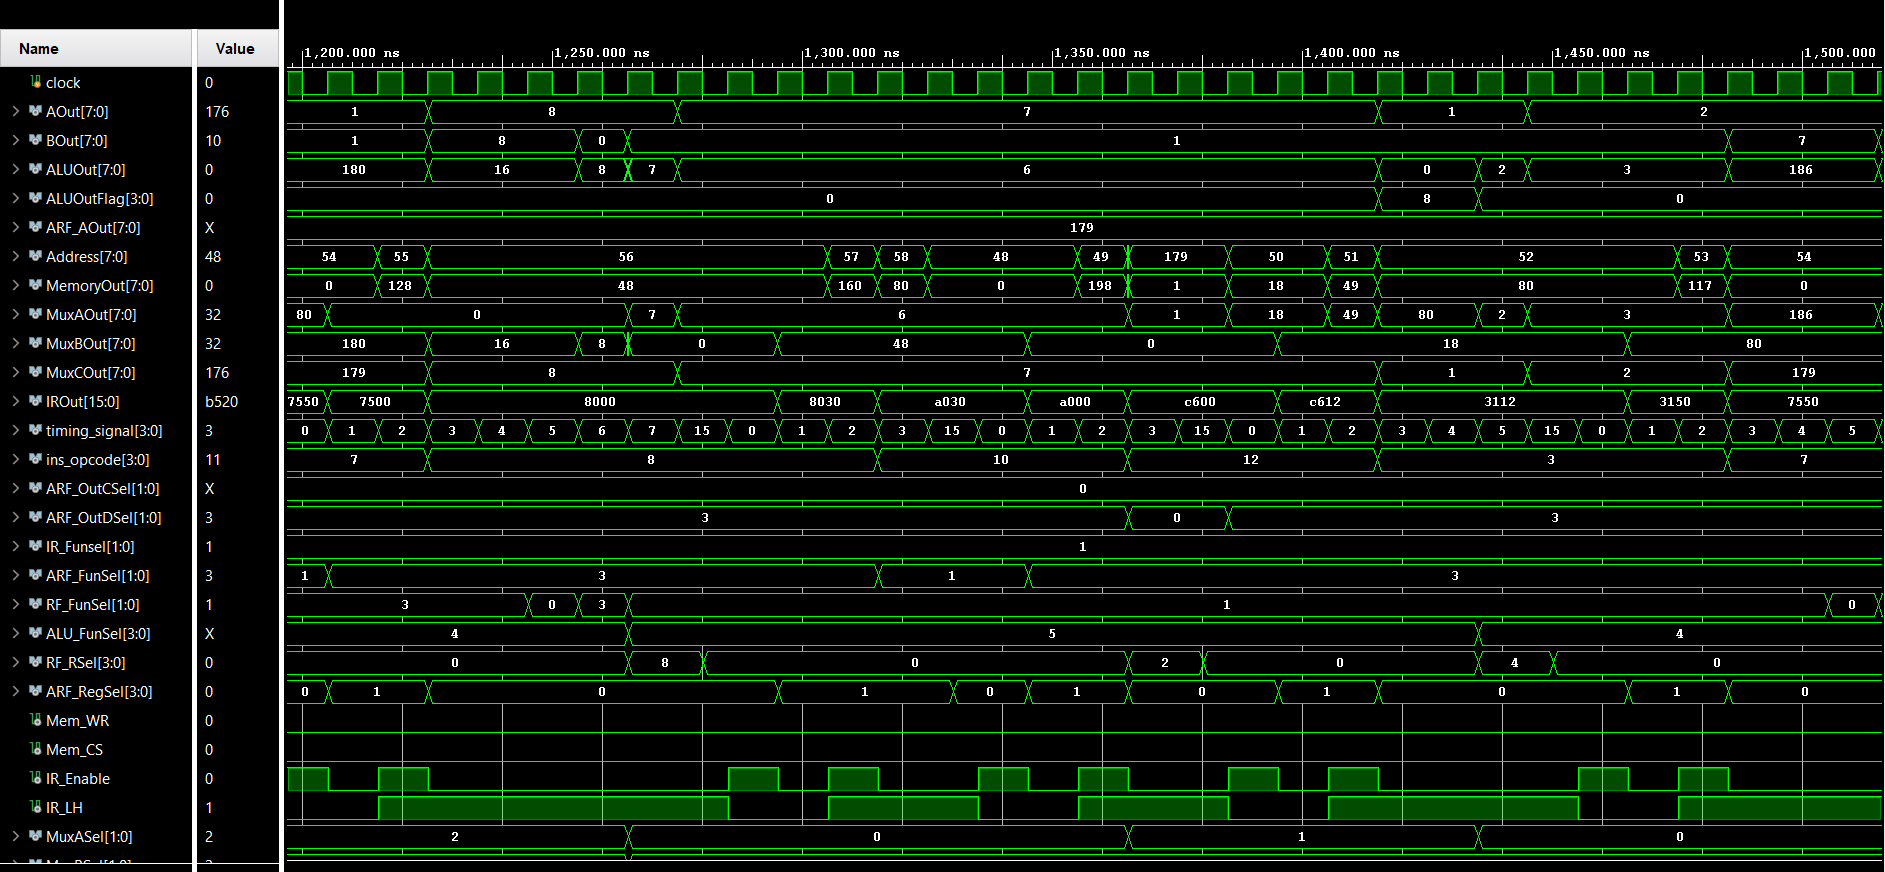
\includegraphics[width=1\textwidth]{photos/system_result_5.png}	
    \caption{simulation of system}
    \label{implementation}
\end{figure}


\begin{figure}[H]
    \centering
    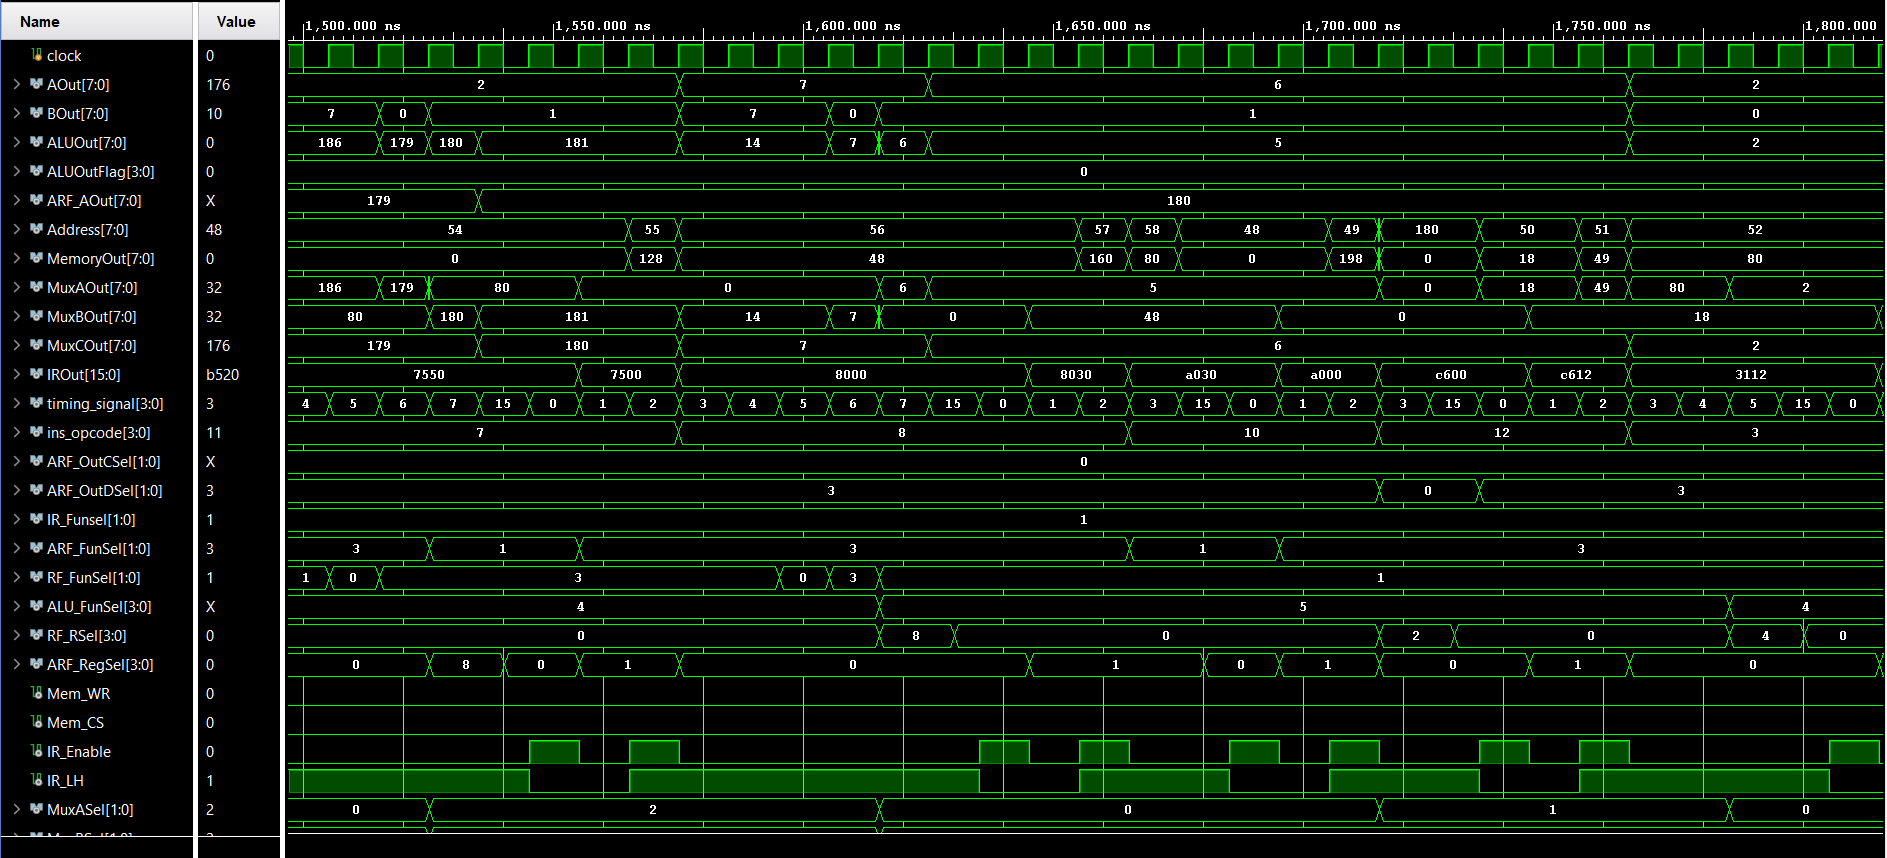
\includegraphics[width=1\textwidth]{photos/system_result_6.png}	
    \caption{simulation of system}
    \label{implementation}
\end{figure}


\begin{figure}[H]
    \centering
    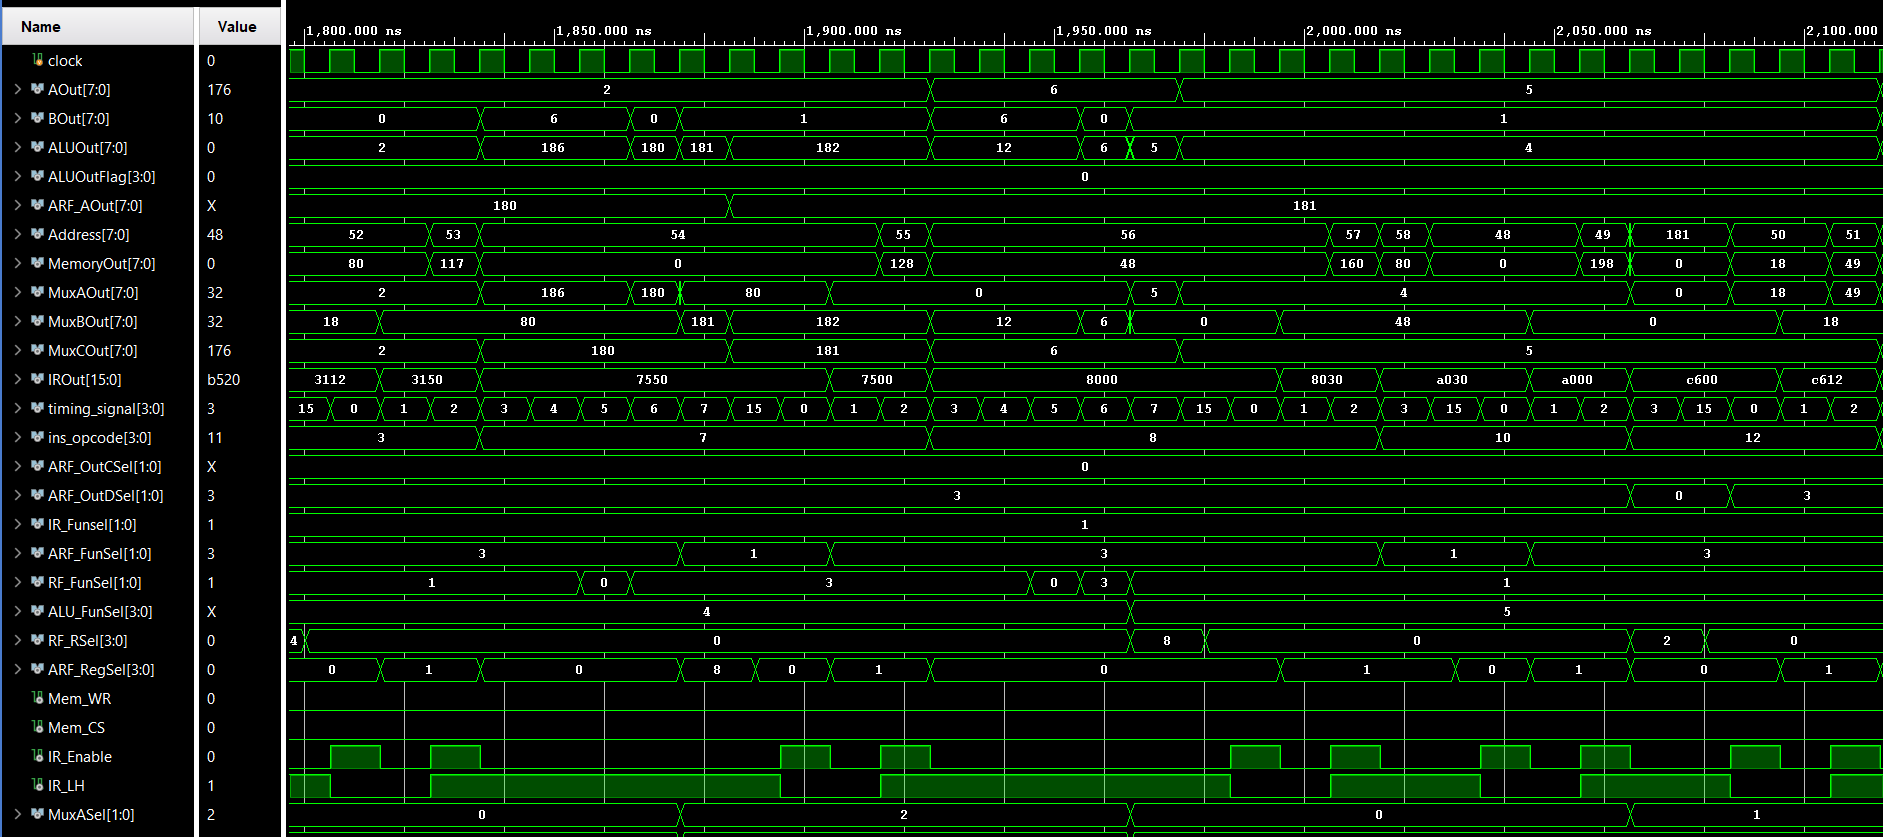
\includegraphics[width=1\textwidth]{photos/system_result_7.png}	
    \caption{simulation of system}
    \label{implementation}
\end{figure}

\begin{figure}[H]
    \centering
    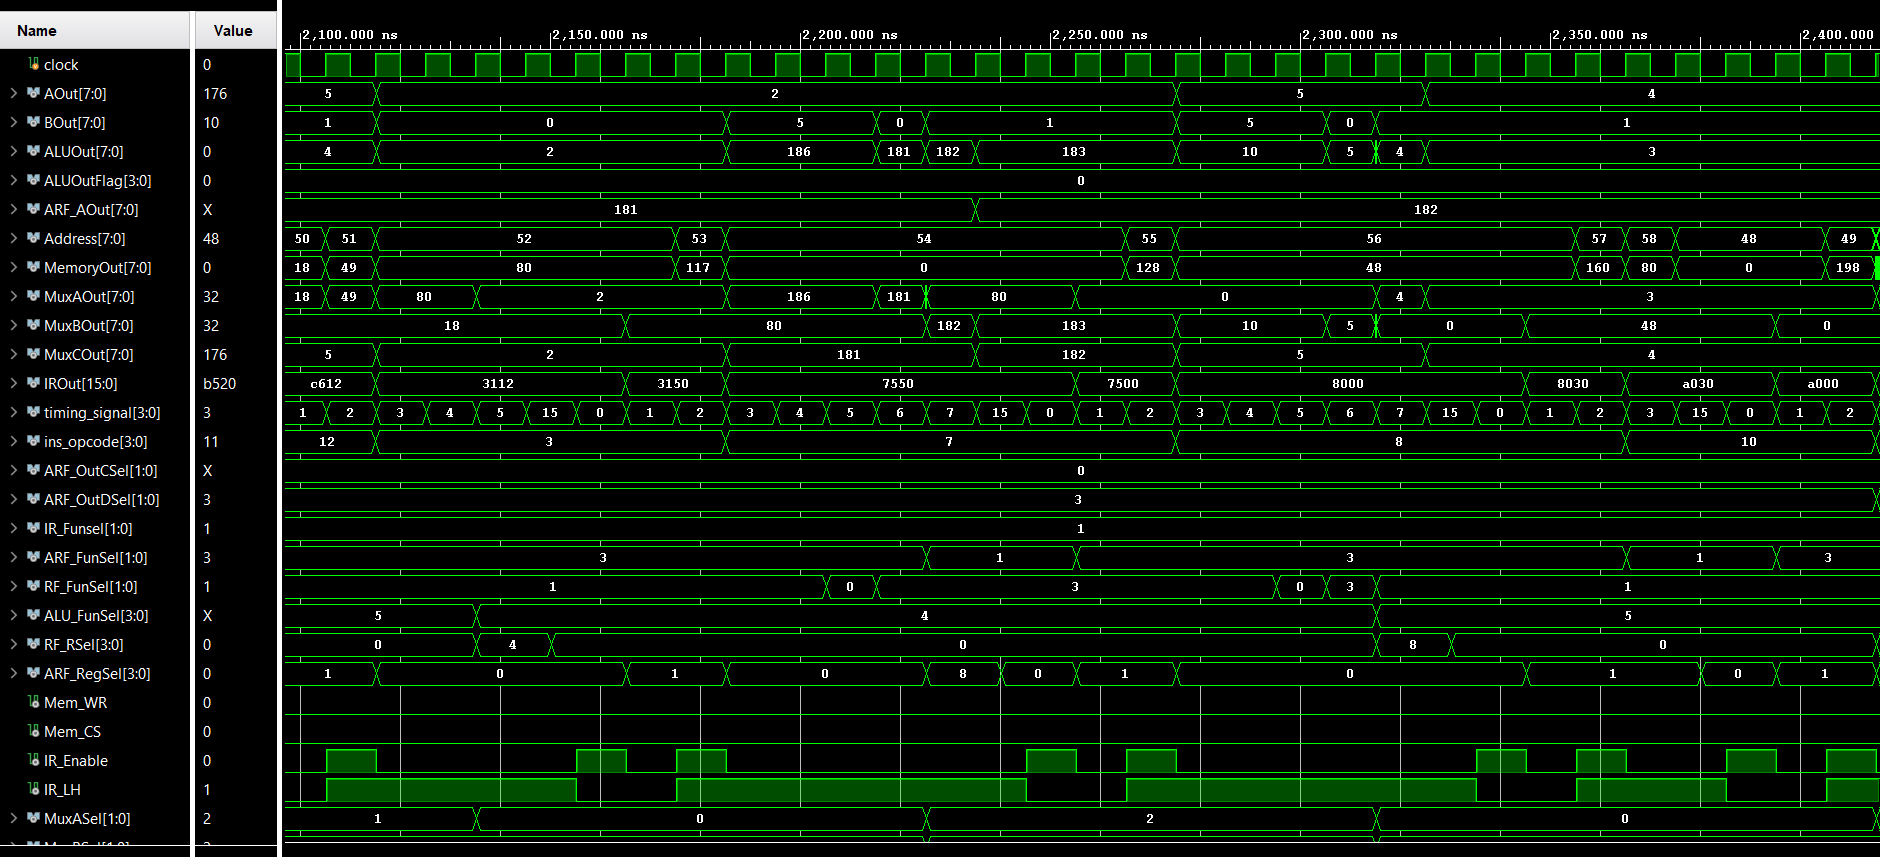
\includegraphics[width=1\textwidth]{photos/system_result_8.png}	
    \caption{simulation of system}
    \label{implementation}
\end{figure}

\begin{figure}[H]
    \centering
    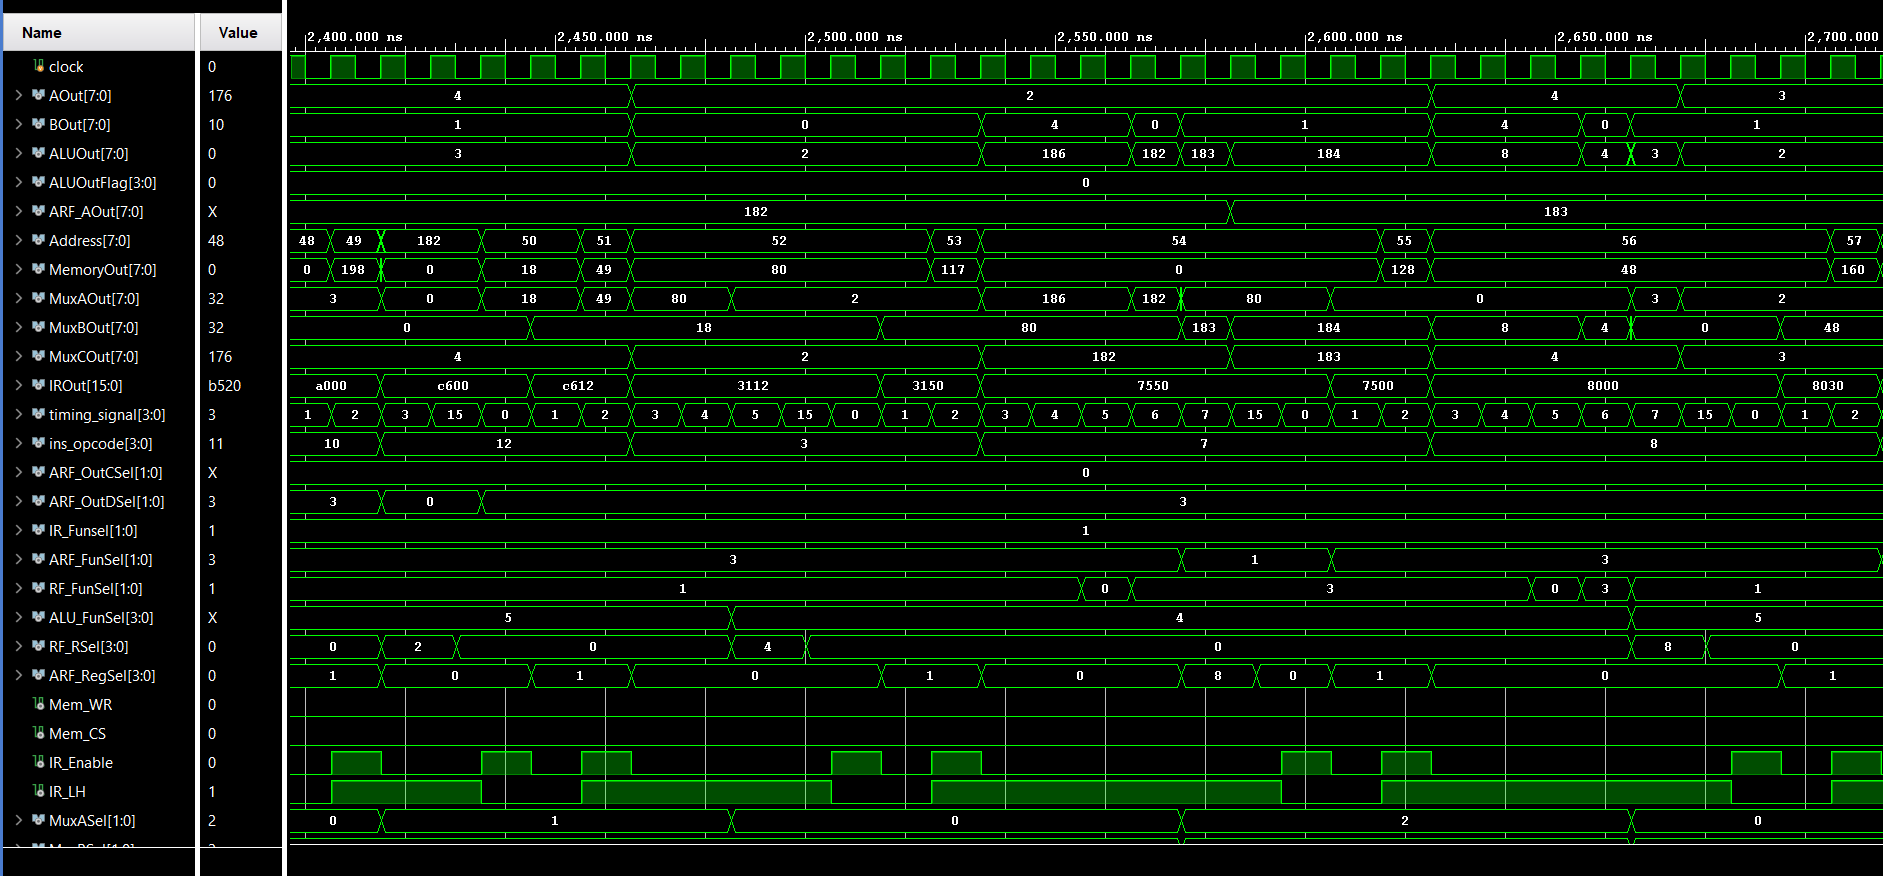
\includegraphics[width=1\textwidth]{photos/system_result_9.png}	
    \caption{simulation of system}
    \label{implementation}
\end{figure}

\begin{figure}[H]
    \centering
    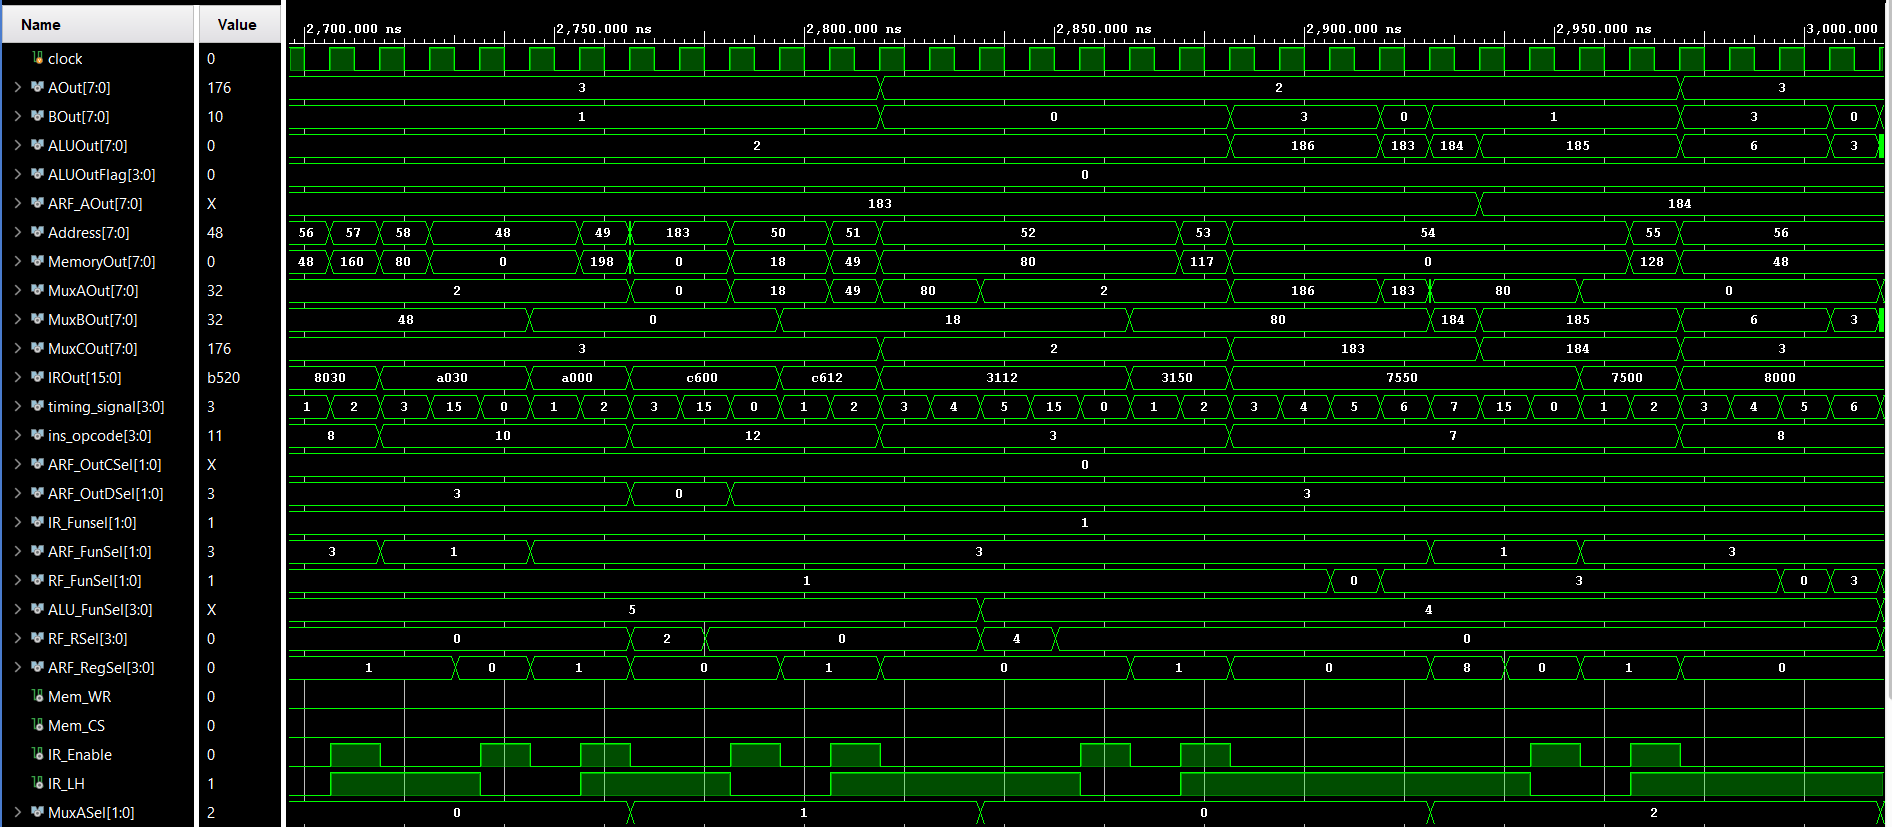
\includegraphics[width=1\textwidth]{photos/system_result_10.png}	
    \caption{simulation of system}
    \label{implementation}
\end{figure}

\begin{figure}[H]
    \centering
    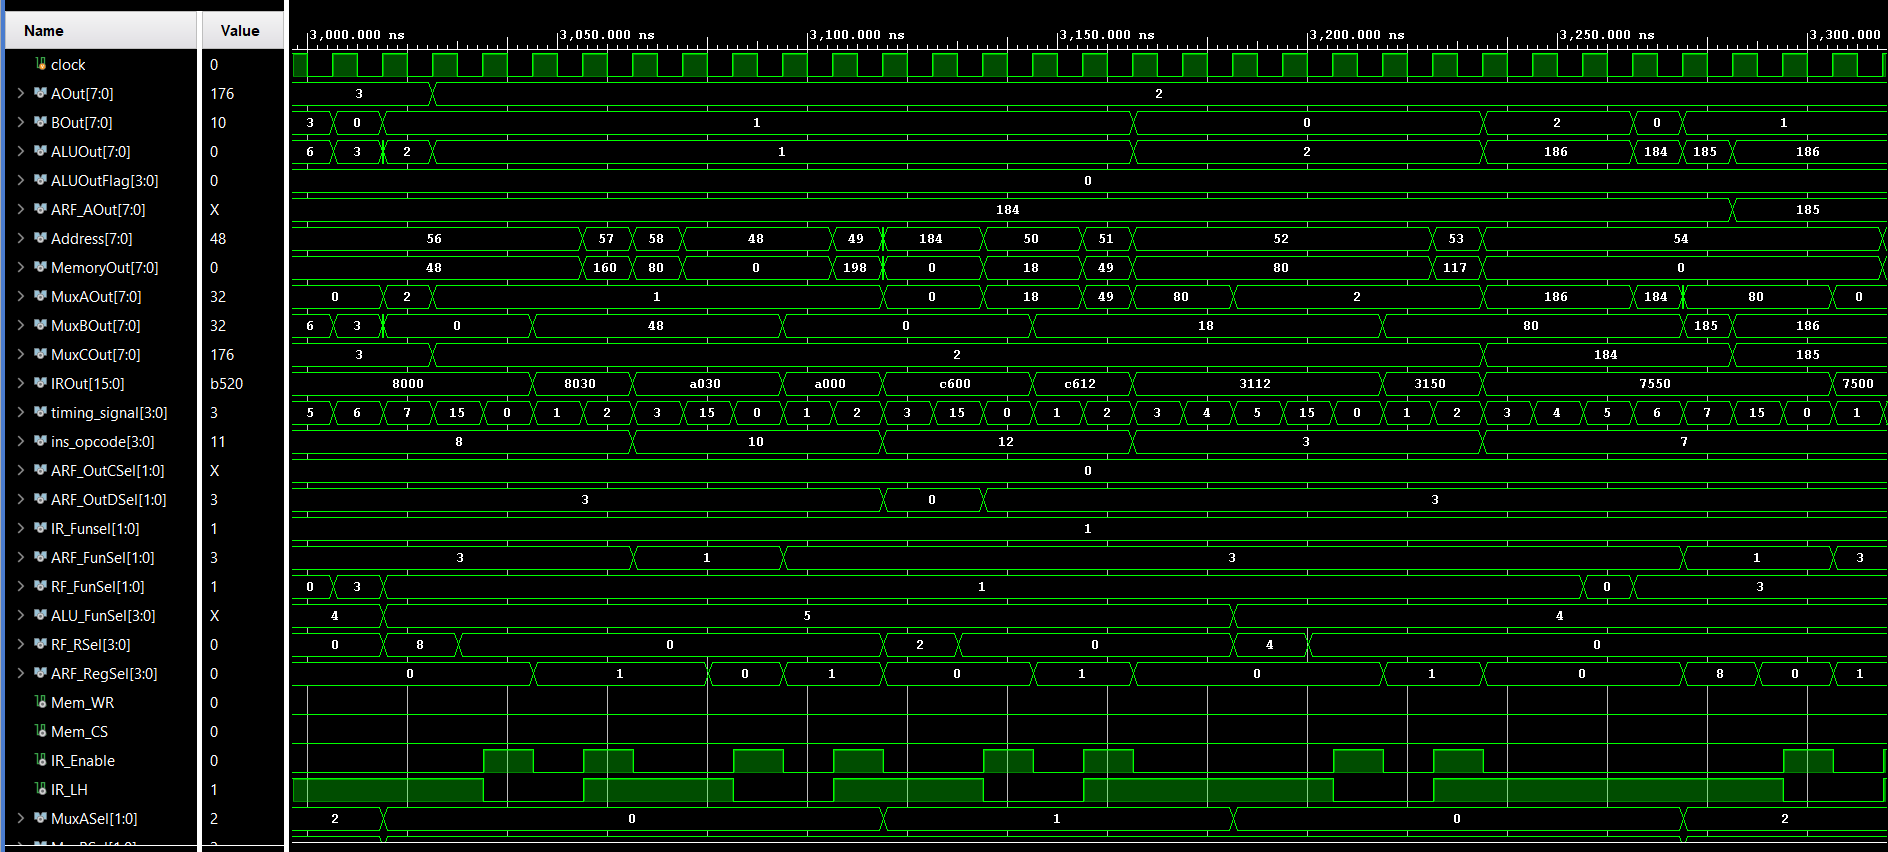
\includegraphics[width=1\textwidth]{photos/system_result_11.png}	
    \caption{simulation of system}
    \label{implementation}
\end{figure}

\begin{figure}[H]
    \centering
    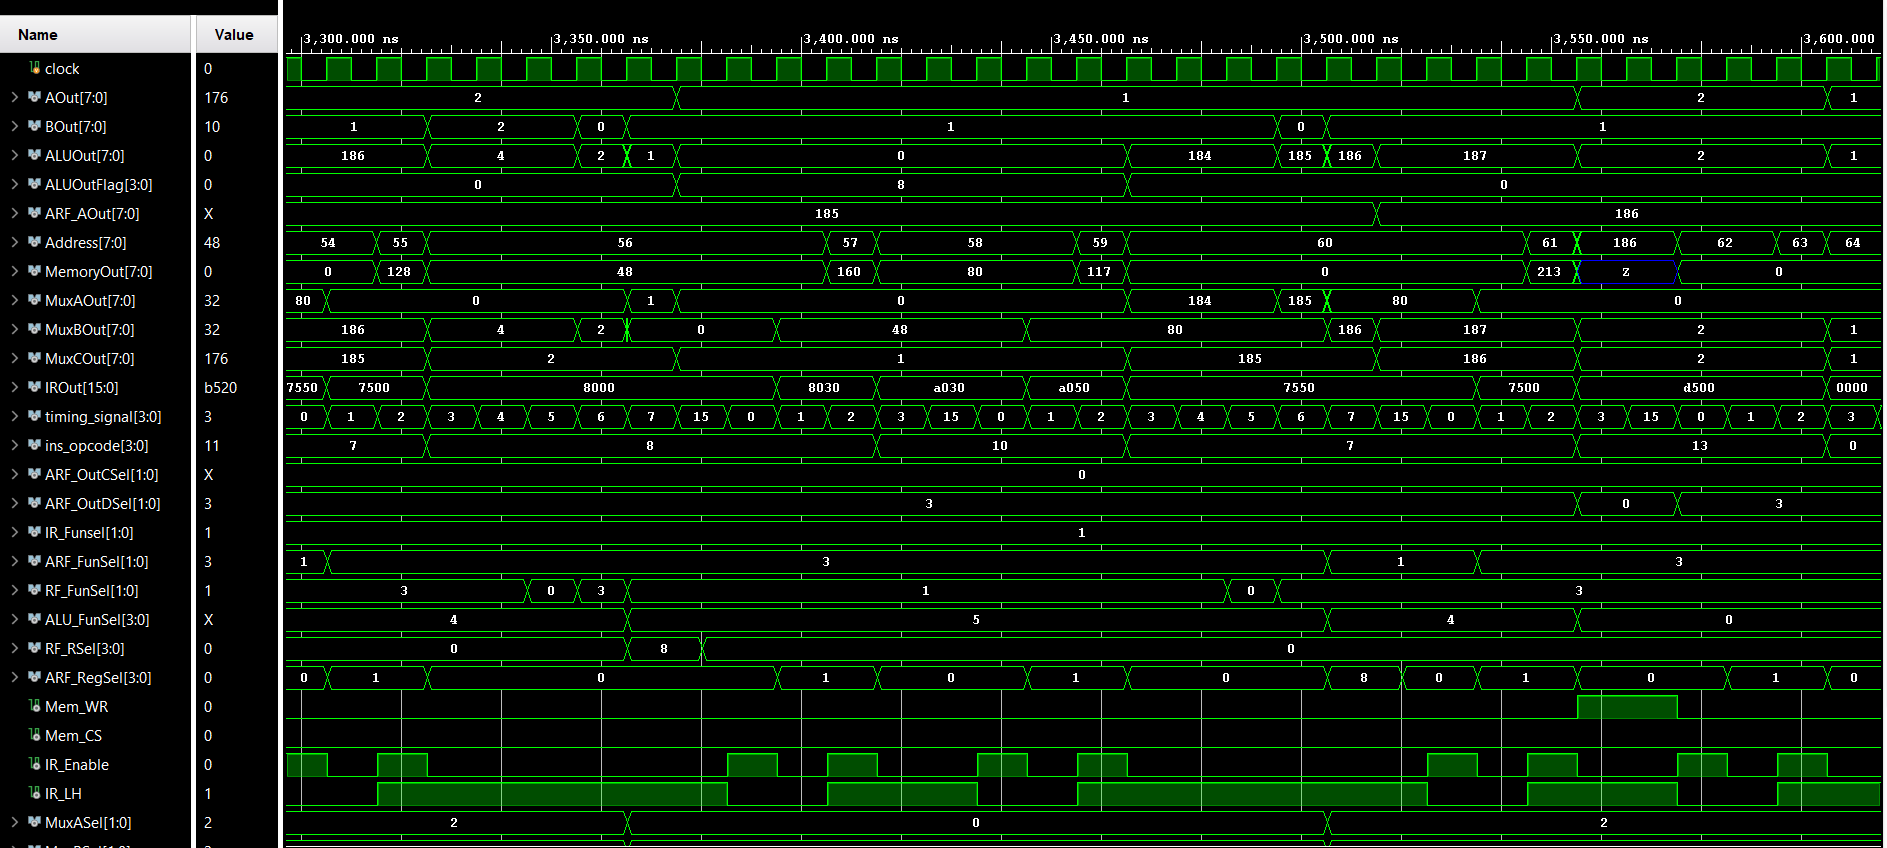
\includegraphics[width=1\textwidth]{photos/system_result_12.png}	
    \caption{simulation of system}
    \label{implementation}
\end{figure}

\begin{figure}[H]
    \centering
    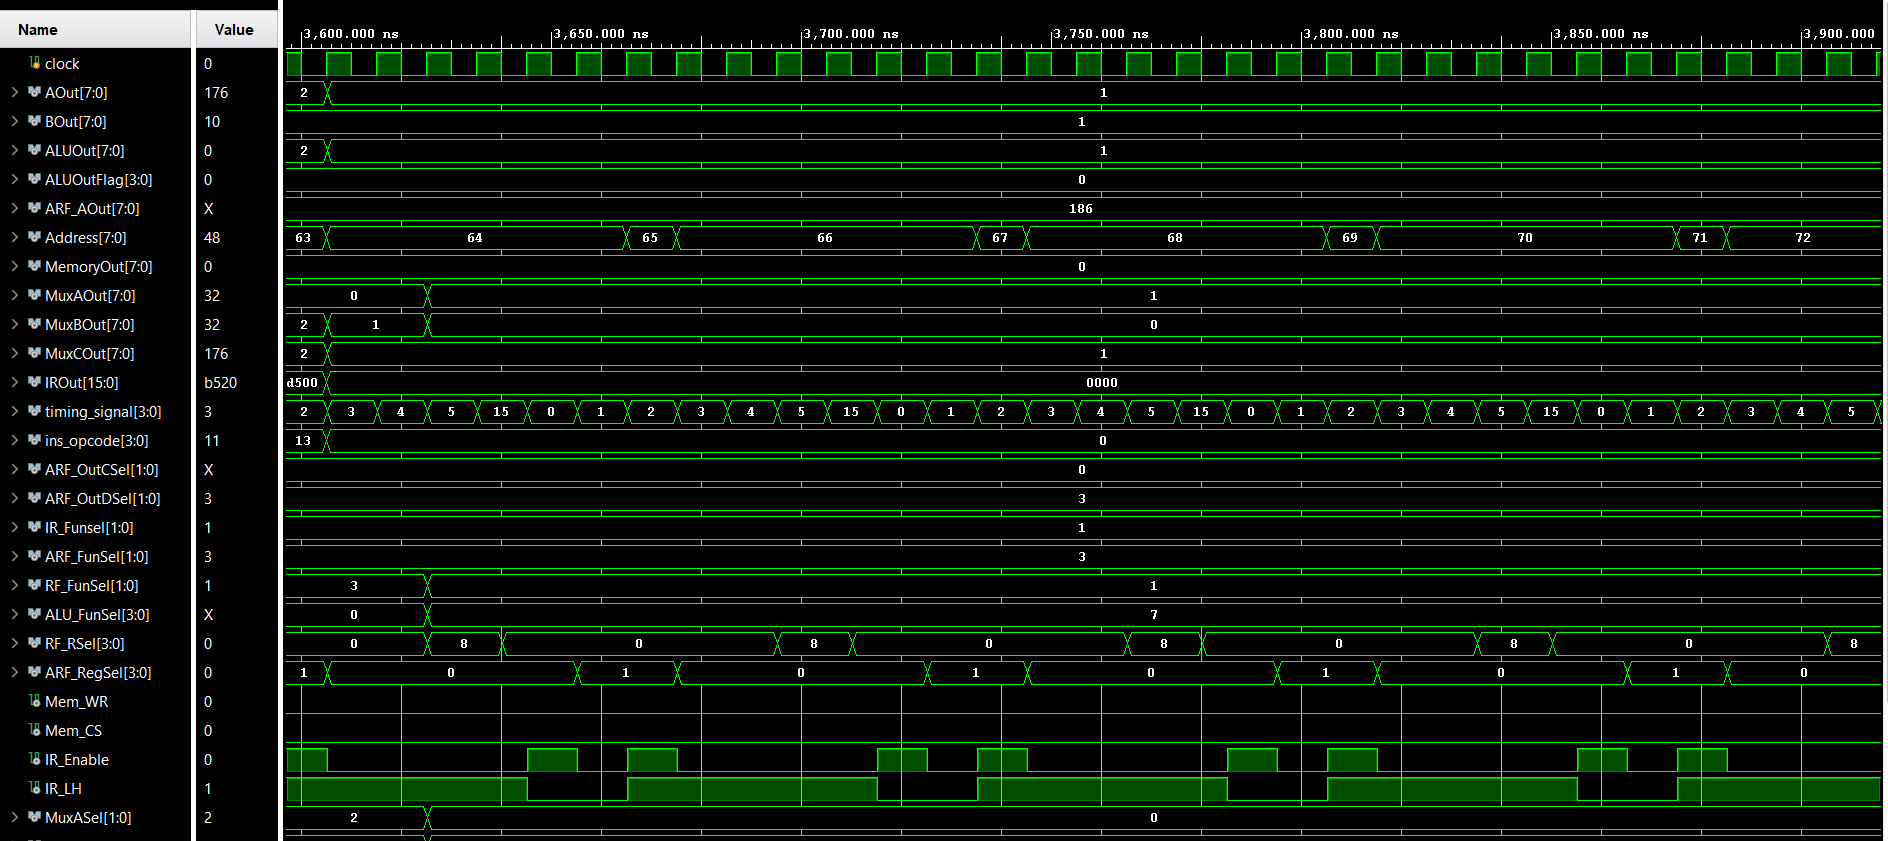
\includegraphics[width=1\textwidth]{photos/system_result_13.png}	
    \caption{simulation of system}
    \label{implementation}
\end{figure}




\section{DISCUSSION}

ilk önce nasıl fetch cycle yaptığından bahset. 




\section{CONCLUSION}
In this project we designed a hardwired control unit with the help of the ones we created in the first project. 

\end{document}